\documentclass[a4paper]{article}

\usepackage[top=1.5cm,bottom=1.5cm,left=2.5cm,right=2.5cm]{geometry}
\usepackage[czech]{babel}
\usepackage{graphicx}

\title{\Huge Parní Sčítačka\\\huge Uživatelská příručka}
\author{\LARGE tým Parní mlátičky \\ Marek Havel \\ Ondřej Zobal\\ Vladimír Hucovič\\ Petr Kolouch}
\date{\today}

\begin{document}

\maketitle

Vážený uživateli, děkujeme, že jste si zvolil právě náš produkt. Pro nejlepší možný zážitek při instalaci a používání naší kalkulačky prosím pozorně čtěte instrukce v tomto dokumentu.

\section*{Instalace, odinstalace}

\subsection*{Instalace pomocí před-sestaveného balíčku (doporučeno)}

Instalaci provádí jednoduchý skript, který stáhne závislosti pro sestavení, sestaví aplikaci a poskládá vhodné soubory na vhodná místa.

Stáhněte celý základní repozitář, vstupte do něj, dále do složky src a v této složce spusťte soubor installer.sh z nadřazeného adresáře:

\verb|../installer.sh|

Instalátor požaduje oprávnění administrátora, aby mohl doinstalovat závislosti a sestavit program. Instalátor předpokládá přítomnost příkazu \verb|sudo|.

\subsection*{Manuální sestavení a instalace}

Ve zkratce: instalace závislostí, vstoupení do složky src, sestavení, zkopírování binárky, přidání záznamu o aplikaci.

\verb|sudo apt install git qtdeclarative5-dev qt5-qmake g++|

\verb|cd (adresar-programu)/src|

\verb|make|

\verb|cp ../build/gui/gui /usr/bin/parni-scitacka|

\verb|chmod a+x /usr/bin/parni-scitacka|

\verb|cp meta/parni-scitacka.desktop ~/.local/share/applications|

\verb|cp meta/parni-scitacka.xpm /usr/share/pixmaps/|

\subsection*{Odinstalace předinstalovaného balíčku}

Odinstalace je prováděna spuštěním odinstalačního skriptu.

Pro odinstalační skript stačí vstoupit do základní složky repozitáře a spustit jej:

\verb|./uninstall.sh|

Pro odinstalaci jsou potřeba práva administrátora.

\subsection*{Manuální odinstalace}

Odinstalace je v podstatě prostě smazání pár věcí z konkrétních složek:

\verb|rm /usr/bin/parni-scitacka|

\verb|rm ~/.local/share/applications/parni-scitacka.desktop|

\verb|rm /usr/share/pixmaps/parni-scitacka.xpm|

\pagebreak

\section*{Jak používat Parní Sčítačku}

\begin{figure}[ht]
	\begin{center}
		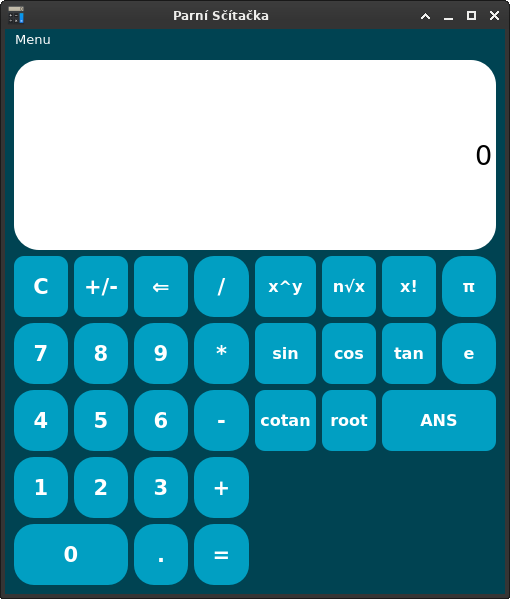
\includegraphics[scale=0.55]{../screenshot.png}
		\caption{Uživatelské rozhraní Parní Sčítačky}
	\end{center}
\end{figure}

Základem používání kalkulačky je vložení nějaké hodnoty. Pro vepsání číslic lze použít tlačítka na obrazovce nebo klávesy 0-9, a to jak na numerické, tak na alfanumerické části klávesnice. 
Desetinnou \textit{tečku} lze vložit tlačítkem \verb|.| jak na obrazovce, tak na klávesnici.
Znaménko nenulové hodnoty lze nastavit pomocí tlačítka \verb|+/-| nebo klávesou \verb|N|.
Pro smazání poslední zapsané číslice lze použít tlačítko $\Leftarrow$ na obrazovce nebo klávesu backspace.

Operace, které požadují pouze jednu hodnotu, lze vyvolat jak před, tak po zadání čísla.

Funkce kalkulačky jsou k dispozici na následujících klávesách:

\begin{tabular}{|c|c|}
\hline
Funkce & Klávesa \\
\hline
$x + y$ & + \\
$x - y$ & - \\
$x \cdot y$ & * \\
$x : y$ & / \\
$x^y$  & U \\
$\sqrt[n]{x}$ & R \\
$n!$ & F \\
$\pi$ & P \\
$e$ & E \\
$\sin{x}$ & S \\
$\cos{x}$ & C \\
$\tan{x}$ & T \\
\textit{ans} & A \\
\hline
\end{tabular}\\

Výsledek lze získat zmáčknutím klávesy \verb|=| na obrazovce.

\end{document}
